Part 2: Unsupervised Feature Selection\\
Question 2.1:\\	
\textsl{Using your clustering method(s) of choice, find a suitable clustering for the cells. Briefly explain how you chose the number of clusters by appropriate visualizations and/or numerical findings.}\\

Answer:\\
As the "elbow" plot indicates, there are different cluster sizes which might fit to this case. Another tool to test the number of clusters for the data is the silhouette plot or the average silhouette score as a summarization of multiple silhouette plots (see figure \ref{fig:silhouette_elbow}). In general, the average silhouette score is quite low. For 3 clusters we achieve an average silhouette score of 0.3 which corresponds to the "elbow" of the "elbow" plot. In the range between 17 to 36 clusters we achieve a comparably high average silhouette score. But due to this wide range, we should not pick one number, especially with these low scores in general.\\

\begin{figure}[h]
	\centering
	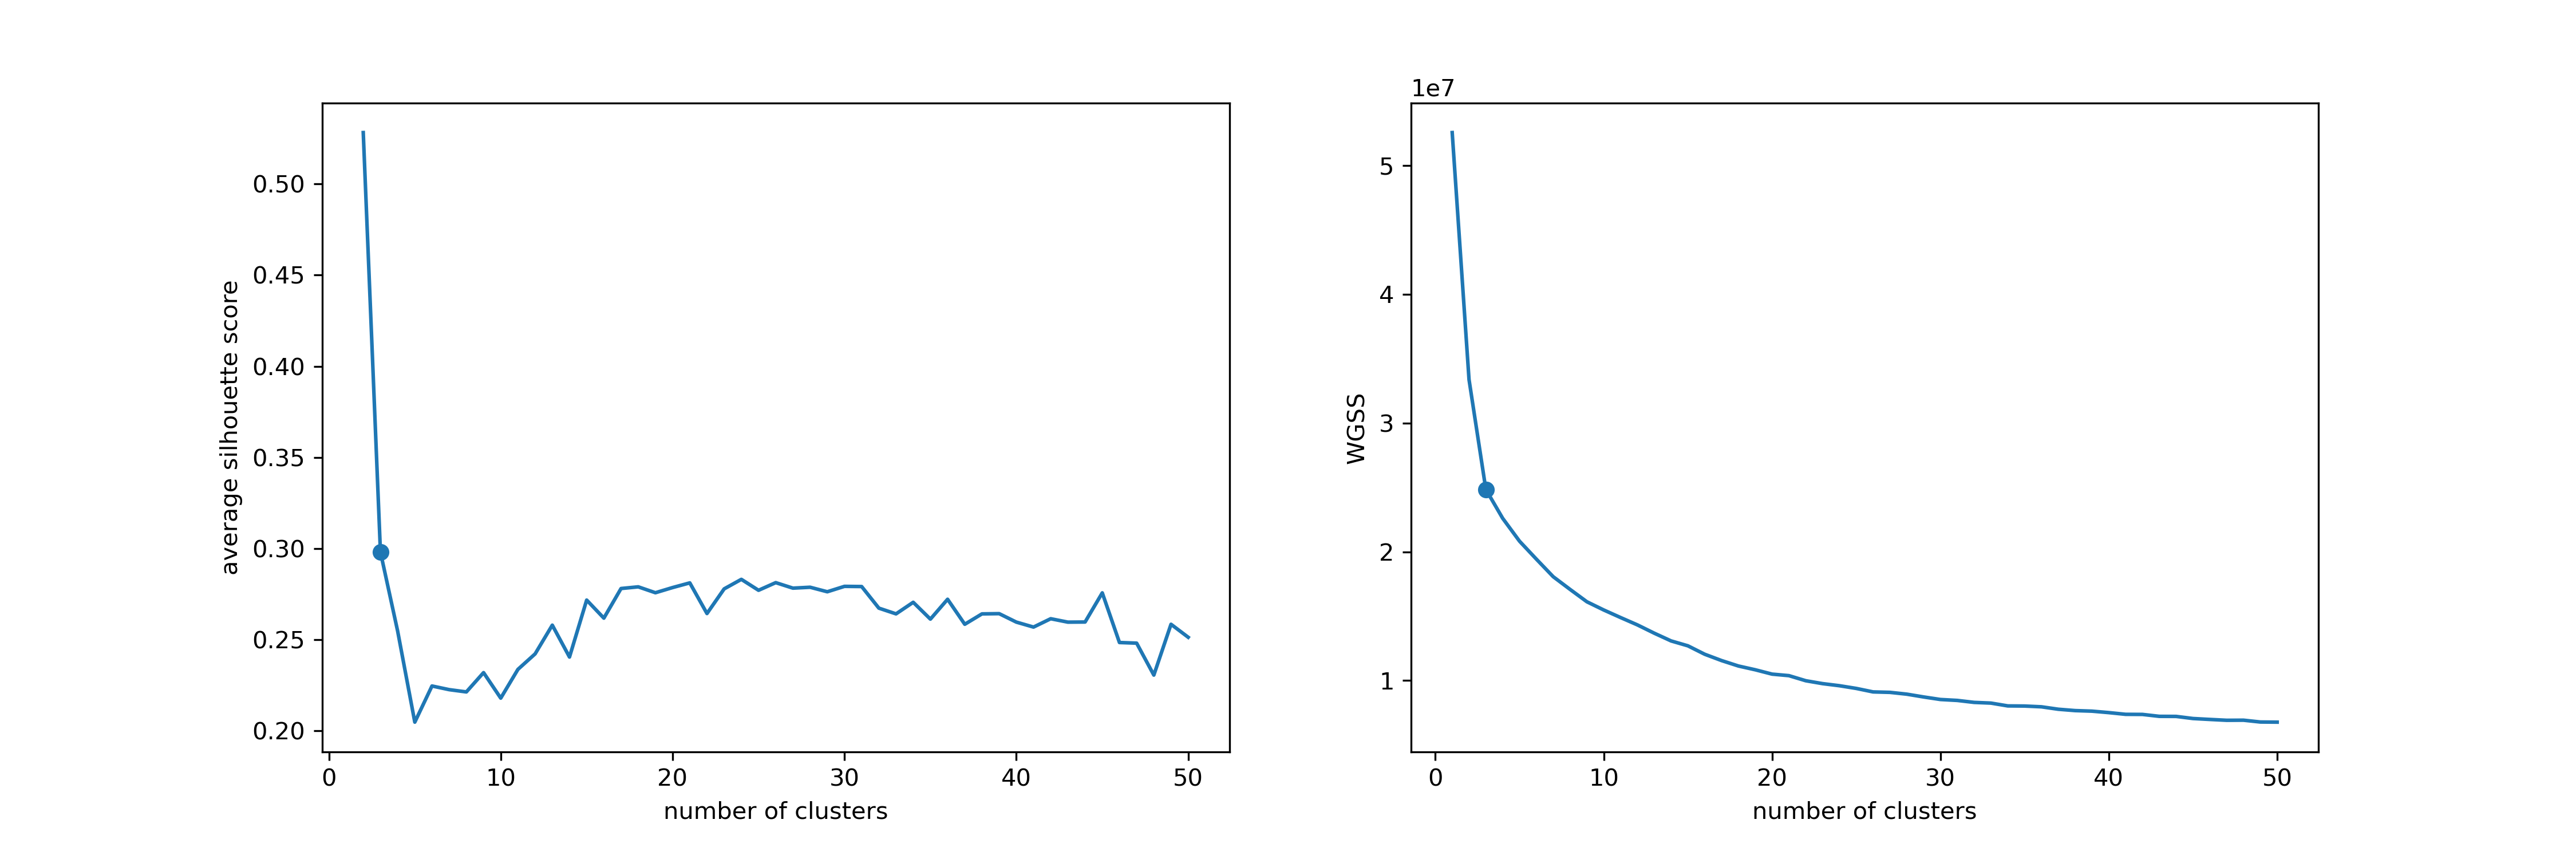
\includegraphics[width=1\linewidth]{problem_02/silhouette_elbow}
	\caption{Average silhouette score (left) and "elbow" plot (right) over number of clusters}
	\label{fig:silhouette_elbow}
\end{figure}

Therefore, the next considerations will focus on 3 clusters. This is supported by the information we have so far (e.g. by scientist's statement).\\

As seen in problem 1.1, we can easily plot 3 clusters in different plots, which makes the differentiation more robust (see figure \ref{fig:clusters})\\